\begin{definition}
If the limit $$\lim_{h\to0}\frac{f(x+h)-f(x)}{h}$$ exists, the function $f$ is \textbf{differentiable}.
\end{definition}

\begin{example}
An example of a function which is not differentiable at a certain point:
\begin{equation*}
f(x)=|x|=
\begin{cases}
\,\,\,\,\, x\quad x\ge0 \\
-x\quad x<0
\end{cases}.
\end{equation*}

\begin{figure}[H]
\centering
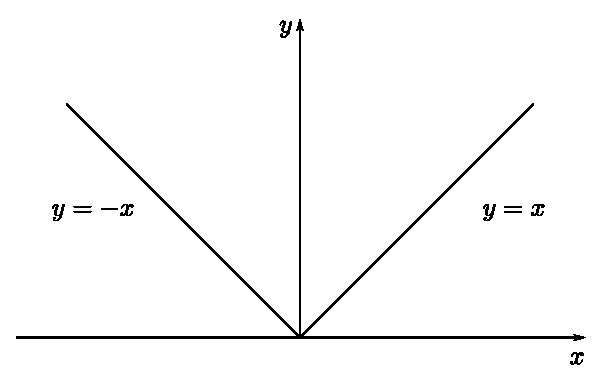
\includegraphics[scale=0.8]{img/mod-x-graph}
\captionstyle{\centering\it}
\caption{Graph of $y=|x|$.}
\label{fig:mod-x-graph}
\end{figure}

At $x=0$, $f(x)$ is continuous but not differentiable, since through the point $(0,0)$, you can draw many, many tangent lines. We can also show
\begin{equation*}
\text{for}\quad h>0,\quad \frac{f(0+h)-f(0)}{h}=\frac{h-0}{h}=1,
\end{equation*}
\begin{equation*}
\text{for}\quad h<0,\quad \frac{f(0+h)-f(0)}{h}=\frac{-h-0}{h}=-1,
\end{equation*}
i.e.
\begin{equation*}
\lim_{h\to0}\frac{f(0+h)-f(0)}{h}
\end{equation*}
doesn't exist! Taking the limit from both sides must give the same answer.
\end{example}

\section{Some common derivatives}

\begin{in_a_box}
The derivative of $x^n$ is $nx^{n-1}$.
\begin{proof}
\begin{eqnarray*}
\frac{df}{dx}&=&\lim_{h\to0}\frac{f(x+h)-f(x)}{h} \\
&=&\lim_{h\to0}\frac{(x+h)^n-x^n}{h} \\
&=&\lim_{h\to0}\frac{\{x^n + nx^{n-1}h+\frac{n(n-1)}{2}x^{n-2}h^2+\dots+h^{n}\}-x^n}{h} \\
&=&\lim_{h\to0}\left\{ nx^{n-1}+\frac{n(n-1)}{2}x^{n-2}h+\dots+h^{n-1}\right\} \\
&=&nx^{n-1}.
\end{eqnarray*}
\end{proof}
\end{in_a_box}

\begin{in_a_box}
The derivative of $\sin x$ is $\cos x$.
\note{For this to be true, $x$ must be measured in radians.}
\begin{proof}
\begin{eqnarray*}
\frac{df}{dx}&=&\lim_{h\to0}\frac{f(x+h)-f(x)}{h} \\
&=&\lim_{h\to0}\frac{\sin(x+h)-\sin x}{h} \\
&=&\lim_{h\to0}\frac{\sin x\cos h + \cos x\sin h - \sin x}{h} \\
&&\text{When }h\text{ is small, }\sin h\approx h\text{ and }\cos h\approx 1\text{, so:}\\
&=&\lim_{h\to0}\frac{\sin x + h\cos x - \sin x}{h} \\
&=&\lim_{h\to0}\cos x \\
&=&\cos x
\end{eqnarray*}
\end{proof}
\end{in_a_box}

\begin{in_a_box}
The derivative of $\cos x$ is $-\sin x$.
\note{For this to be true, $x$ must be measured in radians.}
\begin{proof}
\begin{eqnarray*}
\frac{df}{dx}&=&\lim_{h\to0}\frac{f(x+h)-f(x)}{h} \\
&=&\lim_{h\to0}\frac{\cos(x+h)-\cos x}{h} \\
&=&\lim_{h\to0}\frac{\cos x\cos h - \sin x\sin h - \cos x}{h} \\
&=&\lim_{h\to0}\frac{\cos x - h\sin x - \cos x}{h} \\
&=&\lim_{h\to0}-\sin x \\
&=&-\sin x
\end{eqnarray*}
\end{proof}
\end{in_a_box}

\begin{in_a_box}
The derivative of $\tan x$ is $\sec^2 x$.

We will see why this is true later.
\end{in_a_box}

We could continue working through all the functions we would like to differentiate and working out their derivatives, but this take a long time. Instead, there are some rules which we can use to save time.

\section{Rules for differentiation}
There are three key rules we can use to differentiate more complicated functions.

\subsection{The sum rule}
\begin{thing}{The sum rule}

If $f$ and $g$ are differentiable, then
\[\frac{d}{dx}\left( f(x)+g(x)\right)=\frac{d}{dx}\left(f(x)\right)+\frac{d}{dx}\left(g(x)\right)\]
or\[\frac{d}{dx}\left( f(x)+g(x)\right)=f'(x)+g'(x) \]
\end{thing}

\begin{example}
Consider the function $f(x)=\left( x^3+x^4\right)$, then using the above we have
\begin{align*} \frac{d}{dx}\left( x^3+x^4\right)&=\frac{d}{dx}\left( x^3\right)+\frac{d}{dx}\left(x^4\right)\\&=3x^2+4x^3.\end{align*}
\end{example}

If you repeatedly apply the sum rule, you have
\begin{equation*}
\frac{d}{dx}\left( f_1(x) +f_2(x)+\dots +f_n(x)\right)=\frac{d}{dx}\left( f_1(x)\right)+\frac{d}{dx}\left( f_2(x)\right)+\dots +\frac{d}{dx}\left( f_n(x)\right). 
\end{equation*}

\subsection{The product rule}
\begin{thing}{The product rule}
If $f$ and $g$ are differentiable, then
\[\frac{d}{dx}\left( f(x)g(x) \right) = \frac{d}{dx}\left(f(x)\right)g(x) + f(x)\frac{d}{dx}\left(g(x)\right)\]
or
\[\frac{d}{dx}\left( f(x)g(x) \right) = f'(x)g(x) + f(x)g'(x)\]
\end{thing}

\begin{example}
\begin{eqnarray*}
\frac{d}{dx}\left[ (x^2+1)(x^3-1) \right] &=& 2x(x^3-1) + (x^2+1)3x^2 \\
&=& 2x^4-2x+3x^4+3x^2 \\
&=& 5x^4 + 3x^2 - 2x.
\end{eqnarray*}
Here we have put 
\[f(x)=x^2+1\quad \implies \quad f'(x)=2x,\]
and
\[g(x)=x^3-1\quad \implies \quad g'(x)=3x^2.\]
\end{example}

\begin{example}
Consider the derivative of $x^5$, so
\begin{eqnarray*}
\frac{d}{dx}\left(x^5\right) &=& \frac{d}{dx}\left(x^4\cdot x\right)\\
&=& 4x^3\cdot x + x^4\cdot1\\
&=& 5x^4,
\end{eqnarray*}
as expected, since
\[\frac{d}{dx}\left(x^n\right)=nx^{n-1}.\]
Here we have put
\[f(x)=x^4 \quad \implies \quad f'(x)=4x^3,\]
and
\[g(x)=x\quad \implies \quad g'(x)=1.\]
\end{example}

\subsection{The chain rule}
\begin{thing}{The chain rule}
If $f$ and $g$ are differentiable, then
\[\frac{d}{dx}\left( f(g(x) ) \right) = f'(g(x))g'(x)\]
\end{thing}

\begin{example}
Consider the function $y(x)=(x^3+2x)^{10}$. Here we will choose $f(w)=w^{10}$ and $g(x)=x^3+2x$, (so $f'(w)=10w^9$ and $g'(x)=3x^2+2$). Then
\begin{eqnarray*}
\frac{d}{dx}\left(y(x)\right)&=& \frac{d}{dx}\left( (x^3+2x)^{10} \right) \\ 
&=& \frac{d}{dx}\left( f(g(x)) \right) \\
&=&f'(g(x))g'(x) \\
&=&10(x^3+2x)^9\cdot  (3x^2+2).
\end{eqnarray*}
Essentially, what we have done is to substitute $g(x)=x^3+2x$ in our function for $y(x)$, to make the differentiation easier.
\end{example} 

\begin{example}
To find $$\frac{d}{dx}\left(\sin(1+x^2)\right)$$ take $f(w)=\sin w$ and $g(x)=1+x^2$ ($f'(w)=\cos w$ and $g'(x)=2x$).

Then
\begin{align*}
\frac{d}{dx}\left(\sin(1+x^2)\right)&=\frac{d}{dx}\left(f(g(x)\right)\\
&=f'(g(x))g'(x)\\
&=\cos(1+x^2)\cdot2x\\
&=2x\cos(1+x^2)
\end{align*}
\end{example}
